\documentclass[11pt]{beamer}
\usetheme{Warsaw}
\usepackage[utf8]{inputenc}
\usepackage{graphicx}
\usepackage{hyperref}
\setbeamertemplate{footline}[frame number]
\usepackage{booktabs}   % For better-looking horizontal lines
\usepackage{amsmath}    % pour les formules mathématiques
\usepackage{subcaption} % pour les sous-figures

% \usepackage[style=ieee]{biblatex}
% \addbibresource{ref.bib}
% \bibliography{ref.bib}


\title{Analyse de trace de sang}
\subtitle{Projet 3A}
\author{Cléa Han, Yanis Labeyrie et Adrien Zabban}
\date{27 Mars 2024}

\begin{document}

\maketitle

% \section{Données}
\begin{frame}{Classes}
    \begin{table}[ht]
        \centering
        \begin{tabular}{|ll|}
            \hline
            \textbf{Classe des types de trace de sang} &  \\
            \hline
            1- Traces passives & 2- Goutte à Goutte \\
            3- Transfert par contact & 4- Transfert glissé \\
            5- Altération par contact & 6- Altération glissée \\
            7- d'Accumulation & 8- Coulée \\
            9- Chute de volume & 10- sang Propulsé \\
            11- d'éjection & 12- Volume Impacté \\
            13- Imprégnation & 14- Zone d'interruption \\
            15- d'impact & 16- Foyer de modèle d'impact \\
            17- Trace gravitationnelle & 18- Sang expiré \\
            19- Trace d'insecte & \\
            \hline
        \end{tabular}
        \caption{Liste des 19 modèles de trace de sang}
        \label{tab:classes}
    \end{table}
\end{frame}

\begin{frame}{Données}
    \begin{itemize}
        \item 2 datasets: données de laboratoire et données réelles issus de scène de crime
        \item données labo: 10978 images coupés en 80\%, 10\%, 10\%.
        \item données réelles: 245 images coupés en 60\%, 10\%, 30\% de sorte à avoir 70 images dans le test.
    \end{itemize}
\end{frame}

\begin{frame}{Images de laboratoire}
    \begin{figure}[b]
        \centering
        \begin{subfigure}{0.40\textwidth}
            \centering
            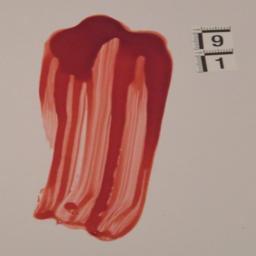
\includegraphics[width=\linewidth]{../asset/data_labo/4_papier_1586.jpg}
            \caption{Modèle Transfert glissé sur un fond de papier}
        \end{subfigure}
        \begin{subfigure}{0.40\textwidth}
            \centering
            \includegraphics[width=\linewidth]{../asset/data_labo/8_coulée_4526.jpg}
            \caption{Modèle de Coulée sur fond de lino}
        \end{subfigure}
        \caption{Deux images de laboratoire}
        \label{fig: labs images}
    \end{figure}
\end{frame}


\begin{frame}{Images réelles}
    \begin{figure}[ht]
        \centering
        \begin{subfigure}{0.40\textwidth}
            \centering
            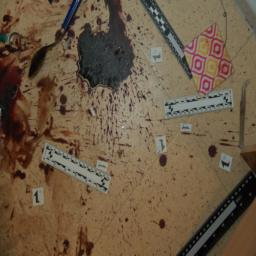
\includegraphics[width=\linewidth]{../asset/data_real/12.jpg}
            \caption{Modèle Volume Impacté}
        \end{subfigure}
        \begin{subfigure}{0.40\linewidth}
            \centering
            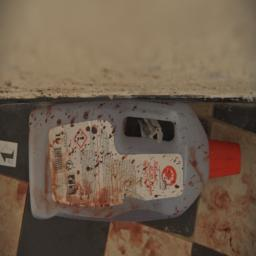
\includegraphics[width=\textwidth]{../asset/data_real/15.jpg}
            \caption{Modèle d'impact}
        \end{subfigure}
        \caption{Deux images de scènes de crime}
        \label{fig: reals images}
    \end{figure}
\end{frame}

\begin{frame}{Data processing}
    \begin{itemize}
        \item reshape en $256\times256$
        \item symétries horizontales et verticales
        \item pas de rotation
        \item changement contraste et la luminescence
        \item pas de data augmentation sur la validation et le test
    \end{itemize}
\end{frame}

% \section{Modèles}
\begin{frame}{Modèle ResNet}
    \begin{itemize}
        \item \textbf{LP ResNet}: Resnet 50 où l'on a remplacé la dernière couche dense de dimension 1000 par deux couches dense avec une dimension de sortie de 18. Et on gèle les autres poids
        \item \textbf{AWL ResNet}: On ne gèle pas les poids.
    \end{itemize}
    \begin{figure}
        \centering
        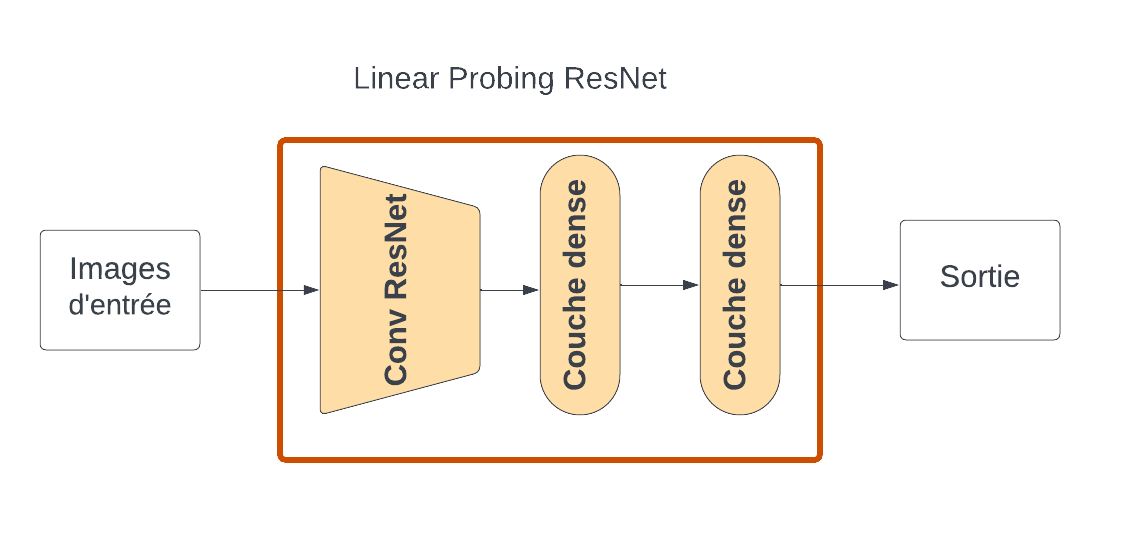
\includegraphics[width=0.7\textwidth]{../asset/Resnet.png}
        \caption{Schéma du modèle LP Resnet}
        \label{fig:resnet}
    \end{figure}
\end{frame}

\begin{frame}{Modèle Adversarial: prédire le background}
    \begin{figure}
        \centering
        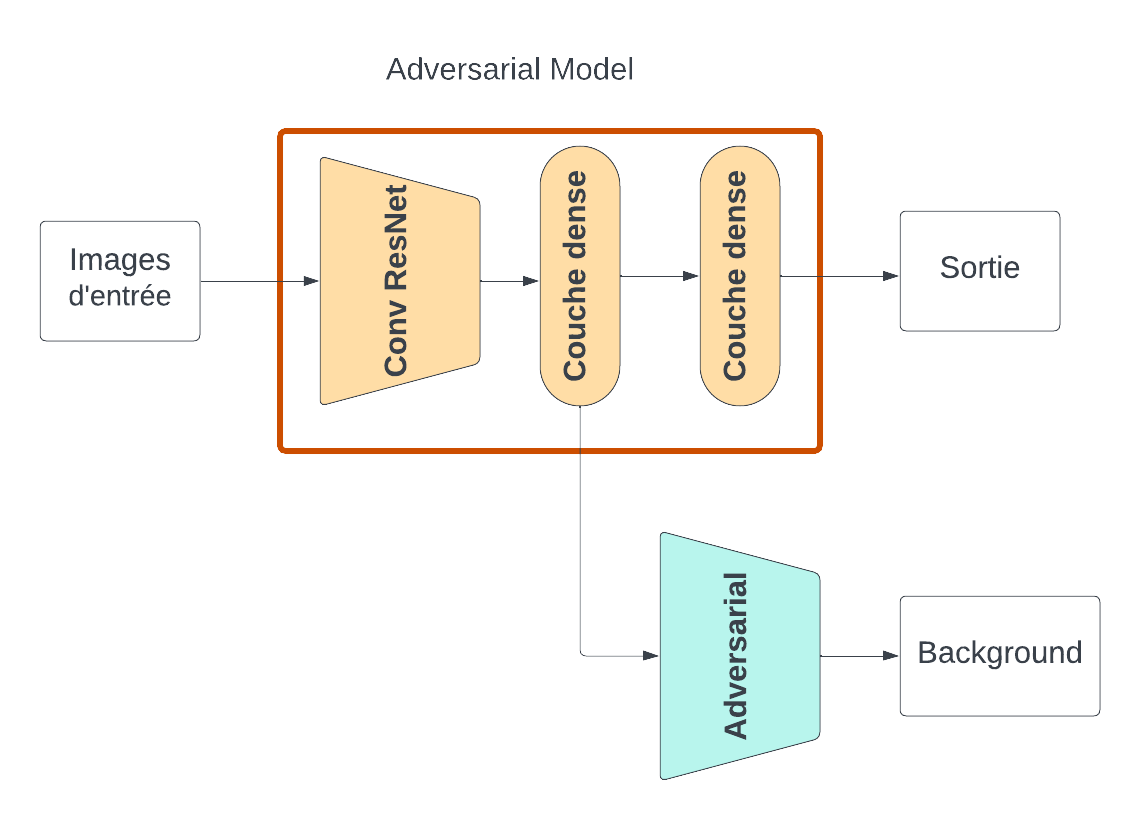
\includegraphics[width=0.6\textwidth]{../asset/Resnet_adv.png}
        \caption{Schéma du modèle Resnet adversarial}
        \label{fig:resnet_adv}
    \end{figure}
    \begin{itemize}
        \item loss utilisé $L_{adv} = \frac{CE_{tache}}{\alpha CE_{background}}$
    \end{itemize}
\end{frame}

\begin{frame}{Modèle Fine Tune}
    \begin{itemize}
        \item Fine Tune des modèles ResNet sur les données réelles
        \item LP Resnet $\rightarrow$ FT LP ResNet
        \item AWL Resnet $\rightarrow$ FT AWL ResNet
    \end{itemize}
\end{frame}

% \section{Métriques}
\begin{frame}{Les Métriques utilisées}
    \begin{itemize}
        \item \textbf{Accuracy micro}: accuracy "classique"
        \item \textbf{Accuracy macro}: moyenne des accuracy sur chacune des classes
        \item Rappel, précision et le f1 score
        \item top k, avec $k=3$
    \end{itemize}
\end{frame}

% \section{Trouver les meilleurs hyperparamètre}
\begin{frame}{Meilleur learning rate}
    \begin{itemize}
        \item Implémentation d'un Grid Search pour trouver le meilleur learning rate pour LP ResNet.
    \end{itemize}
    \begin{table}[ht]
        \centering
        \begin{tabular}{cccccc}
        \toprule
        learning rate & acc micro & acc macro & f1-score & top 3 \\
        \midrule
        0.01 & 85.1 & 78.8 & 78.1 & 49.4 \\
        0.005 & 89.1 & 84.7 & 83.6 & \textbf{52.5} \\
        0.001 & 90.4 & 85.7 & 84.8 & 50.5 \\
        0.0005 & \textbf{91.1} & \textbf{86.8} & \textbf{86.0} & 49.1 \\
        0.0001 & 84.9 & 78.6 & 77.4 & 50.4 \\
        \bottomrule
        \end{tabular}
        \caption{Résultat de validation à la fin des entraînements des modèles LP ResNet avec différents learning rate.}
        \label{tab:gridsearch}
    \end{table}
\end{frame}

\begin{frame}{Trouver les meilleurs hyperparamètres pour Adversarial}
    \begin{table}
        \centering
        \begin{tabular}{cc}
            \toprule
            Paramètres & Valeurs possibles\\
            \midrule
            $lr_{res}$ & 0.01, 0.005, 0.001, 0.005, 0.0001\\
            $lr_{adv}$ & 0.01, 0.005, 0.001, 0.005, 0.0001\\
            $\alpha$ & 0.001, 0.1, 0.5, 1, 2, 5, 10, 100\\
            \bottomrule
        \end{tabular}
        \caption{Liste des valeurs possibles pour les hyperparamètres testés dans le Random Search}
        \label{tab:random search possibilities}
    \end{table}
\end{frame}

\begin{frame}{Trouver les meilleurs hyperparamètres pour Adversarial}
    \begin{table}[ht]
        \centering
        \begin{tabular}{cccccc}
        \toprule
        res acc micro & res acc macro & adv acc micro & $lr_{res}$ & $lr_{adv}$ & $\alpha$ \\
        \midrule
        79.3 & 72.8 & 82.5 & 0.1 & 1 & 10 \\
        89.6 & 84.7 & 16.1 & 0.1 & 1 & 0.1 \\
        \textbf{90.8} & \textbf{86.2} & 20.2 & 0.5 & 0.01 & 0.1 \\
        85.3 & 81.2 & 44.6 & 0.1 & 1 & 0.5 \\
        88 & 85.7 & 72 & 0.5 & 0.5 & 2 \\
        89.4 & 85.4 & 56.8 & 0.01 & 0.1 & 0.5 \\
        89.5 & 85.4 & 71 & 0.1 & 0.1 & 1 \\
        87.2 & 82.2 & 71.7 & 1 & 0.01 & 1 \\
        85.3 & 80.3 & \textbf{85.3} & 0.1 & 0.5 & 10 \\
        86.7 & 83.2 & 84.8 & 0.1 & 0.01 & 10 \\
        \bottomrule
        \end{tabular}
        \caption{Résultat de validation à la fin des entraînements des modèles Adversarial avec différents hypermaramètres.}
        \label{tab:random search results}
    \end{table}
\end{frame}

\begin{frame}{Résultats de test sur les données de labo}
    \begin{table}[ht]
      \centering
        \begin{tabular}{cccccc}
        \toprule
        Modèles & Acc Micro & Acc Macro & F1-score & Top 3 \\
        \midrule
        LP ResNet & 95.2 & 94.3 & 94.7 & \textbf{99.8} \\
        AWL ResNet & \textbf{97.3} & \textbf{97.1} & \textbf{96.2} & \textbf{99.8} \\
        Adversarial & 93.4 & 91.8 & 91.8 & \textbf{99.8} \\
        \bottomrule
        \end{tabular}
        \caption{Résultats de test sur les données de laboratoire}
        \label{tab:results_lab}
    \end{table}
\end{frame}

\begin{frame}{Résultats de test sur les données de réelles}
    \begin{table}[ht]
      \centering
        \begin{tabular}{ccccccc}
        \toprule
        Modèles & Acc Micro & Acc Macro & F1-score & Top 3 \\
        \midrule
        LP ResNet & 12.9 & 6.0 & 4.0 & 19.0 \\
        FT LP ResNet & 11.8 & 6.1 & 6.4 & 26.0 \\
        AWL Resnet & 17.2 & 13.8 & 8.1 & 28.7 \\
        FT AWL ResNet & \textbf{41.9} & \textbf{33.4} & \textbf{26.9} & \textbf{51.7} \\
        Adversarial & 11.8 & 5.7 & 3.7 & 16.7 \\
        \bottomrule
        \end{tabular}
        \caption{Résultats de test sur les données réelles}
        \label{tab: results_real}
    \end{table}
\end{frame}

\begin{frame}{Cartes de saillance}
    \begin{itemize}
        \item Utilisation de GRAD CAM pour trouver les cartes de saillance.
    \end{itemize}
    \begin{figure}[ht]
        \centering
        \begin{subfigure}{0.40\textwidth}
            \centering
            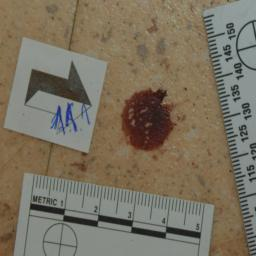
\includegraphics[width=\linewidth]{../asset/exemple/14.jpg}
        \end{subfigure}
        \begin{subfigure}{0.40\textwidth}
            \centering
            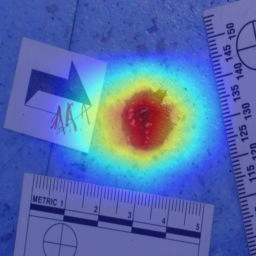
\includegraphics[width=\linewidth]{../asset/exemple/14_saliency.png}
        \end{subfigure}
        \caption{Exemple d'une image  de trace de sang (à gauche) avec sa carte de chaleur Grad CAM superposée (à droite).}
        \label{fig:grad_cam_example}
    \end{figure}
\end{frame}

\begin{frame}{Cartes de saillances}
    \begin{figure}[ht]
        \centering
        \begin{subfigure}{0.40\textwidth}
            \centering
            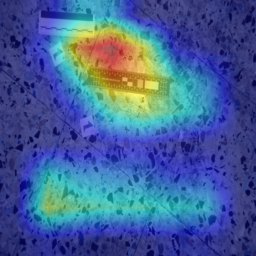
\includegraphics[width=\linewidth]{../asset/exemple/attention_reglette.jpg}
        \end{subfigure}
        \begin{subfigure}{0.40\textwidth}
            \centering
            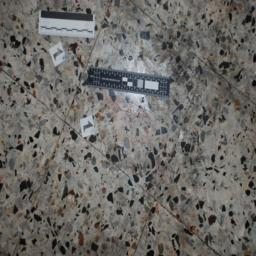
\includegraphics[width=\linewidth]{../asset/exemple/attention_reglette_image.jpg}
        \end{subfigure}
        \caption{Exemple d'une image de trace de sang (à droite) avec sa carte de chaleur Grad CAM superposée (à gauche), dans le cadre d'une attention portée à la réglette.}
        \label{fig:grad_cam reglette}
    \end{figure}
\end{frame}

\begin{frame}{Métriques sur les cartes de saillance}
    \textbf{Average Drop (AD)}
    \begin{equation}
        \text{AD} = \frac{1}{N} \sum_{i=1}^{N} \frac{[p_i - o_i]_+}{p_i} \cdot 100
    \end{equation}
    
    \textbf{Average increase (AI)}
    \begin{equation}
        \text{AI} = \frac{1}{N} \sum_{i=1}^{N} 1_{p_i<o_i} \cdot 100
    \end{equation}
    
    \textbf{Average Gain (AG)}
    \begin{equation}
        \text{AG} = \frac{1}{N} \sum_{i=1}^{N} \frac{[o_i - p_i]_+}{1 - p_i} \cdot 100
    \end{equation}
\end{frame}

\begin{frame}{Métriques sur les cartes de saillance}
    \begin{table}[ht]
        \centering
        \begin{tabular}{cccc}
            \toprule
            Métriques & Average Drop & Average Increase & Average Gain \\
            \midrule
            AWL ResNet & 91.6 & 0.0& 0.0\\
            FT AWL ResNet & 87.6 & 0.0 & 0.0\\
            \bottomrule
            \end{tabular}
        \caption{Résultats des métriques sur les données réelles (de la base de données de test).}
        \label{tab:saliency_results}
    \end{table}

    \begin{itemize}
        \item On a $\forall i \in [1, N], p_i < o_i$
        \item utiliser des méthodes de saliency maps plus performantes comme Grad-CAM++ ou Score-CAM.
    \end{itemize}
\end{frame}

\begin{frame}{Conclusion}
    \begin{itemize}
        \item Bon potentiel: 97\% d'accuracy (micro) contre 41\% avec les données réelles, sachant qu'il y a 10 000 images de laboratoire contre 254 images réelles.
        \item Tentative d'utiliser une clé de détermination
        \item Utiliser un plus gros ResNet
        \item Faire du self-supervise learning pour traiter toutes les données de l'expert
        \item Installer le code chez l'expert pour qu'il puisse le faire tourner en local sur sa machine
        \item Mise à disposition d'un GitHub public pour les prochaines équipes
    \end{itemize}
\end{frame}

\begin{frame}{Annexes: courbe d'apprentissage: LP ResNet}
    \begin{figure}[ht]
        \centering
        \begin{subfigure}{0.32\textwidth}
            \centering
            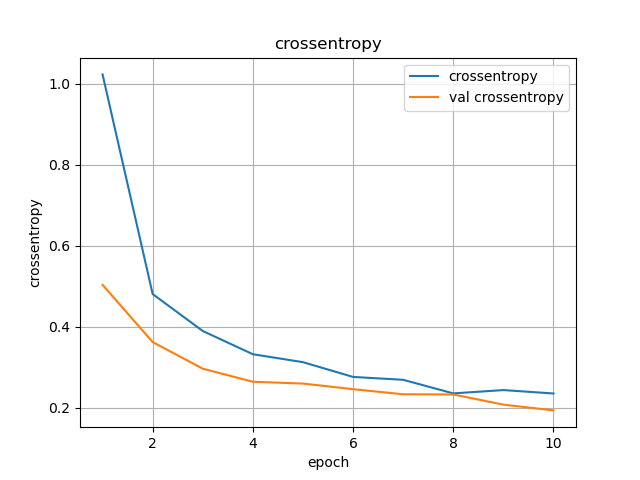
\includegraphics[width=\linewidth]{../logs/resnet_img256_0/crossentropy.png}
            \caption{crossentropy}
        \end{subfigure}
        \begin{subfigure}{0.32\textwidth}
            \centering
            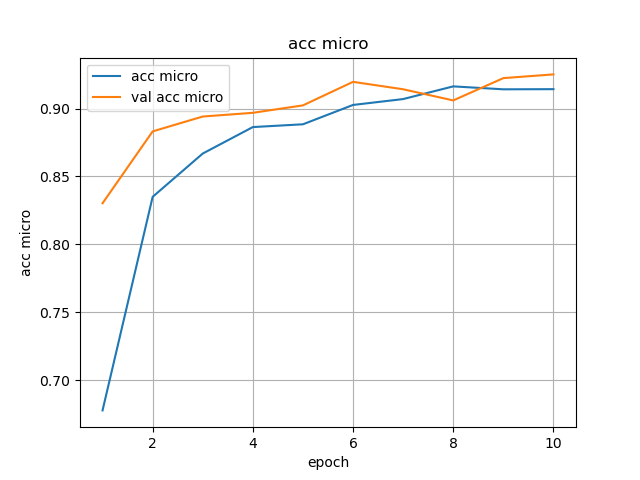
\includegraphics[width=\linewidth]{../logs/resnet_img256_0/acc micro.png}
            \caption{acc micro}
        \end{subfigure}
        \begin{subfigure}{0.32\textwidth}
            \centering
            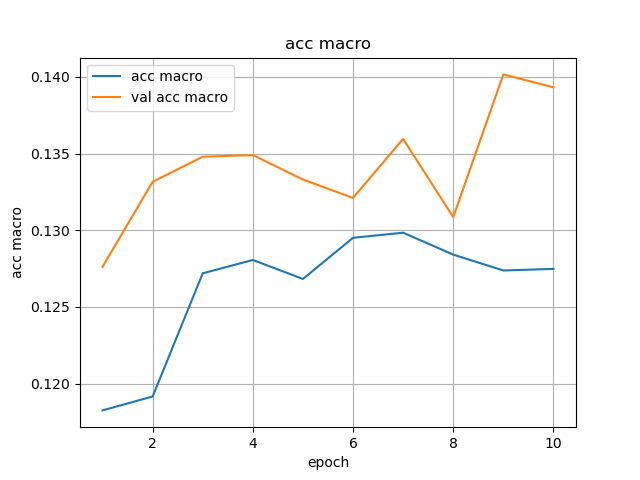
\includegraphics[width=\linewidth]{../logs/resnet_img256_0/acc macro.png}
            \caption{acc macro}
        \end{subfigure}
        \caption{Valeurs de la loss et des accuracy d'entraînement (en bleue) et de validation (en orange) en fonction des epochs durant l'entraînement du modèle LP ResNet.}
        \label{fig: train LP ResNet}
    \end{figure}
\end{frame}

\begin{frame}{Annexes: courbe d'apprentissage: AWL ResNet}
    \begin{figure}[ht]
        \centering
        \begin{subfigure}{0.32\textwidth}
            \centering
            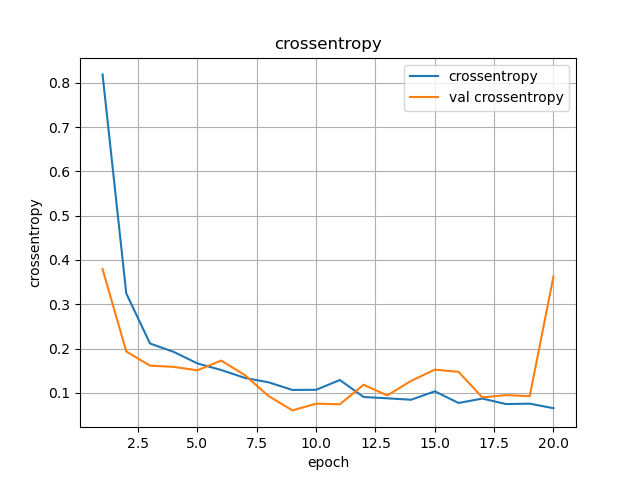
\includegraphics[width=\linewidth]{../logs/resnet_allw_img256_2/crossentropy.png}
            \caption{Crossentropy}
        \end{subfigure}
        \begin{subfigure}{0.32\textwidth}
            \centering
            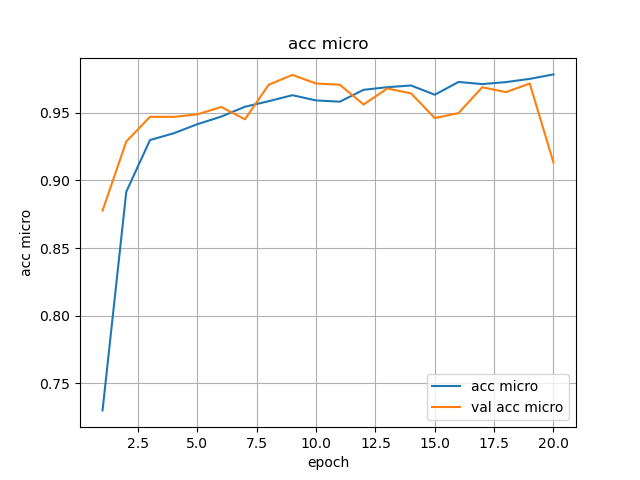
\includegraphics[width=\linewidth]{../logs/resnet_allw_img256_2/acc micro.png}
            \caption{acc micro}
        \end{subfigure}
        \begin{subfigure}{0.32\textwidth}
            \centering
            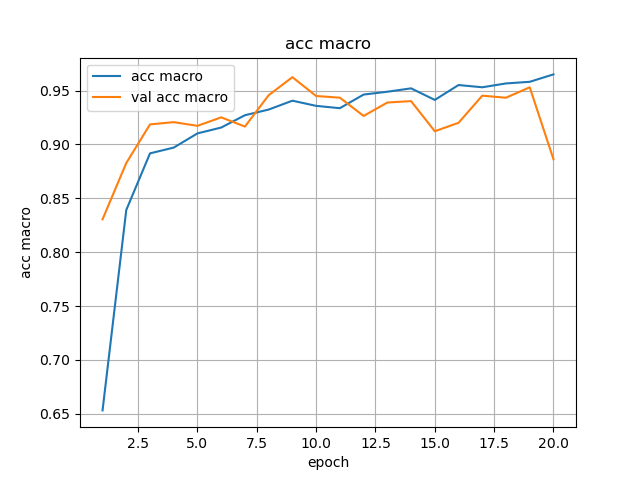
\includegraphics[width=\linewidth]{../logs/resnet_allw_img256_2/acc macro.png}
            \caption{acc macro}
        \end{subfigure}
        \caption{Valeurs de la loss et des accuracy d'entraînement (en bleue) et de validation (en orange) en fonction des epochs durant l'entraînement du modèle AWL ResNet.}
        \label{fig: train AWL ResNet}
    \end{figure}
\end{frame}

\begin{frame}{Annexes: courbe d'apprentissage: Adversarial}
    \begin{figure}[ht]
        \centering
        \begin{subfigure}{0.32\textwidth}
            \centering
            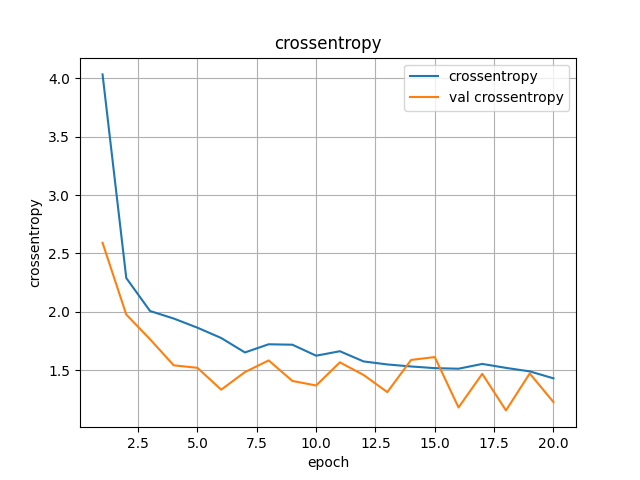
\includegraphics[width=\linewidth]{../logs/adv_img256_1/crossentropy.png}
            \caption{Loss $L_{adv}$}
        \end{subfigure}
        \begin{subfigure}{0.32\textwidth}
            \centering
            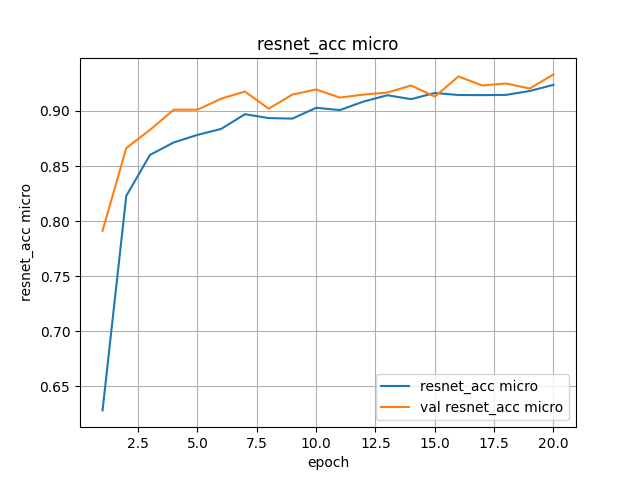
\includegraphics[width=\linewidth]{../logs/adv_img256_1/resnet_acc micro.png}
            \caption{res acc micro}
        \end{subfigure}
        \begin{subfigure}{0.32\textwidth}
            \centering
            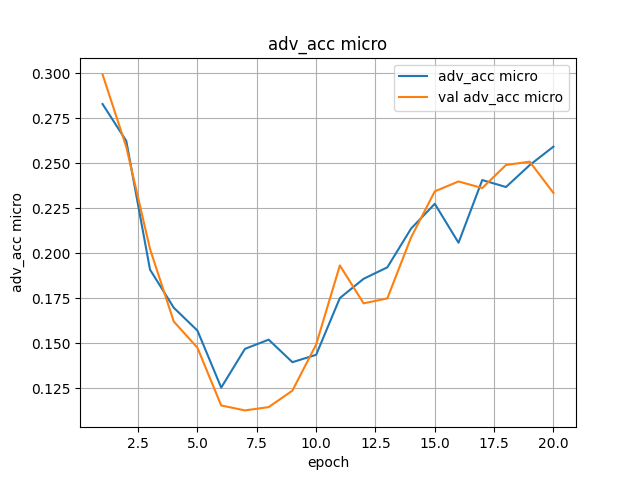
\includegraphics[width=\linewidth]{../logs/adv_img256_1/adv_acc micro.png}
            \caption{adv acc micro}
        \end{subfigure}
        \caption{Valeurs de la loss et des accuracy d'entraînement (en bleue) et de validation (en orange) en fonction des epochs durant l'entraînement du modèle Adversarial.}
        \label{fig: train adv}
    \end{figure}
\end{frame}

\begin{frame}{Annexes: courbe d'apprentissage: FT ResNet}
    \begin{figure}[ht]
        \centering
        \begin{subfigure}{0.45\textwidth}
            \centering
            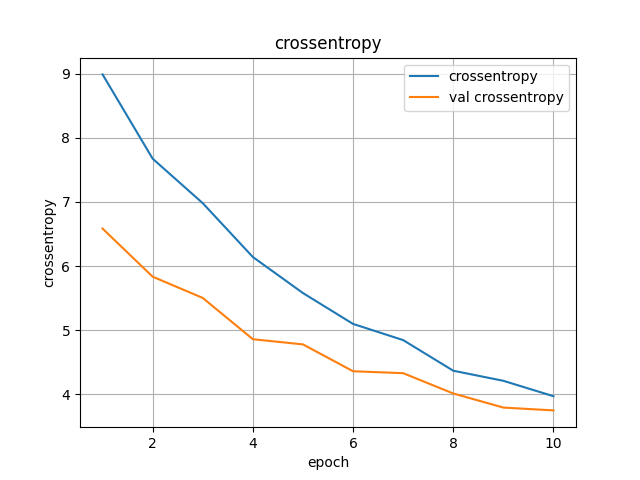
\includegraphics[width=\linewidth]{../logs/retrain_resnet_img256_0/crossentropy.png}
            \caption{crossentropy de FT LP ResNet}
        \end{subfigure}
        \begin{subfigure}{0.45\textwidth}
            \centering
            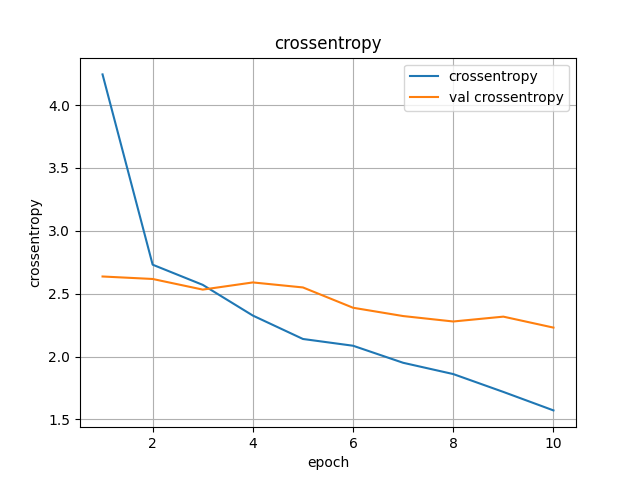
\includegraphics[width=\linewidth]{../logs/retrain_resnet_allw_img256_2/crossentropy.png}
            \caption{crossentropy de FT AWL ResNet}
        \end{subfigure}
        \caption{Valeurs de la loss d'entraînement (en bleue) et de validation (en orange) en fonction des epochs durant l'entraînement des modèles fine-tune sur les données réelles.}
        \label{fig: finetune}
    \end{figure}
\end{frame}

% \begin{frame}{Références}
%     \printbibliography
% \end{frame}


\end{document}

